\documentclass[a4paper,12pt]{article}
\usepackage[T1]{fontenc}
\usepackage[utf8]{inputenc}
\usepackage{graphicx}
\usepackage{amsmath}
\usepackage{amsfonts}
\usepackage{amssymb}
\usepackage{booktabs}
\usepackage{float}
\usepackage{geometry}
\usepackage[german]{babel}
\usepackage{enumitem}
\usepackage{parskip}
\usepackage{underscore}
\usepackage{hyperref}
% \usepackage{multicol}

\geometry{a4paper, left=25mm, right=25mm, top=20mm, bottom=20mm}

%//[x] TODO: Titelblatt und Inhaltsverzeichnis

\begin{document}
\begin{titlepage}
    \centering
    
\includegraphics[scale = 0.03]{bilder/JKU_Logo.png}\\[1.0 cm]	% JKU Logo
    \textsc{\Large Einführungspraktikum Physik}\\[0.5 cm]	        % LVA Name
    \textsc{\large 1. Versuch}\\[0.5 cm]				            % Versuch Nummer
    \rule{\linewidth}{0.4 mm} \\[0.4 cm]
    { \huge \bfseries Würfeln}\\                                    % Versuch Name
    \rule{\linewidth}{0.4 mm} \\[1.5 cm]
    \begin{minipage}{0.8\textwidth}
        \begin{flushleft} \large
            \emph{Autoren:}\\
            Eva Brandstätter (k12406599)\\
            Tobias Mittermair (k12412801)\\
            \vspace{1cm}
            \emph{Gruppe:}\\
            Freitag Vormittag\\
            \vspace{1cm}
            \emph{Betreuer:}\\
            Gerald Gmachmeir
        \end{flushleft}
        \begin{flushright} \large
            \vspace{8cm}
            \emph{Abgabe:} \\
            \today
        \end{flushright}
    \end{minipage}~

    \vfill
    %\rule{\textwidth}{0.1 mm}
    %\tableofcontents
    
\end{titlepage}

\tableofcontents
\newpage


\section{Einleitung}
%//[x] Einleitung
% Was soll gemessen werden? (Ziel / Motivation / Hypothese / erwartetes Ergebnis)
Das Experiment soll die Häufigkeitsverteilung der möglichen Ergebnisse eines Würfelvorgangs zeigen. 
Außerdem sollen der Mittelwert und die Standardabweichung der gemessenen Ergebnisse circa den statistisch 
berechneten Werten entsprechen. Es wird erwartet, dass eine annähernd gleiche Verteilung festgestellt werden kann.

\section{Grundlagen}
%//[x] Grundlagen
% (kurz!) Was muss ich über die zu messende Größe wissen?
Als Würfel wurde ein Spielwürfel verwendet, welcher vereinfacht als dreidimensionaler Körper mit jeweils sechs gleich
großen quadratischen Seiten beschrieben werden kann. Diese Seitenflächen sind mit den Augenzahlen 1 bis 6 beschriftet. 
Ein Würfelvorgang endet mit einer dieser Seiten nach oben zeigend, der Wert dieser Seite wird als das Würfelergebnis gezählt.

Da jeder möglicher Versuchsausgang bei einem fairen Würfel gleich wahrscheinlich ist, ist ein Würfelversuch ein klassisches 
Beispiel eines Laplace Experiments.

Außerdem ist ein wichtiger Gesichtspunkt, dass die Würfe unabhängig voneinander sind und somit ein Wurf keinen Einfluss auf den 
Ausgang des nächsten hat. Dieser Aspekt ist grundlegend für die statistische Auswertung und Analyse des Zufallsexperiments.


\section{Versuchsbeschreibung}
\subsection{Versuchsaufbau}
%//[x] Versuchsaufbau
% Wie sieht der Versuchsaufbau aus? (Skizze, Anleitung, Geräte, …)

Es wurden ein Karton als Würfelteller und fünf Würfel verwendet, wie in Abbildung \ref{Abb1} ersichtlich. Dabei wurde davon ausgegangen, 
dass sich darunter kein gezinkter Würfel befindet. Zusätzlich wurden alle Würfel zuvor auf Beschädigungen, einheitliche 
Seitenlänge und schätzungsweise homogene Massenverteilung kontrolliert. Ein PC stand bereit, um die Werte zeitgleich zu 
dokumentieren.

\begin{figure}[H]
    \centering
    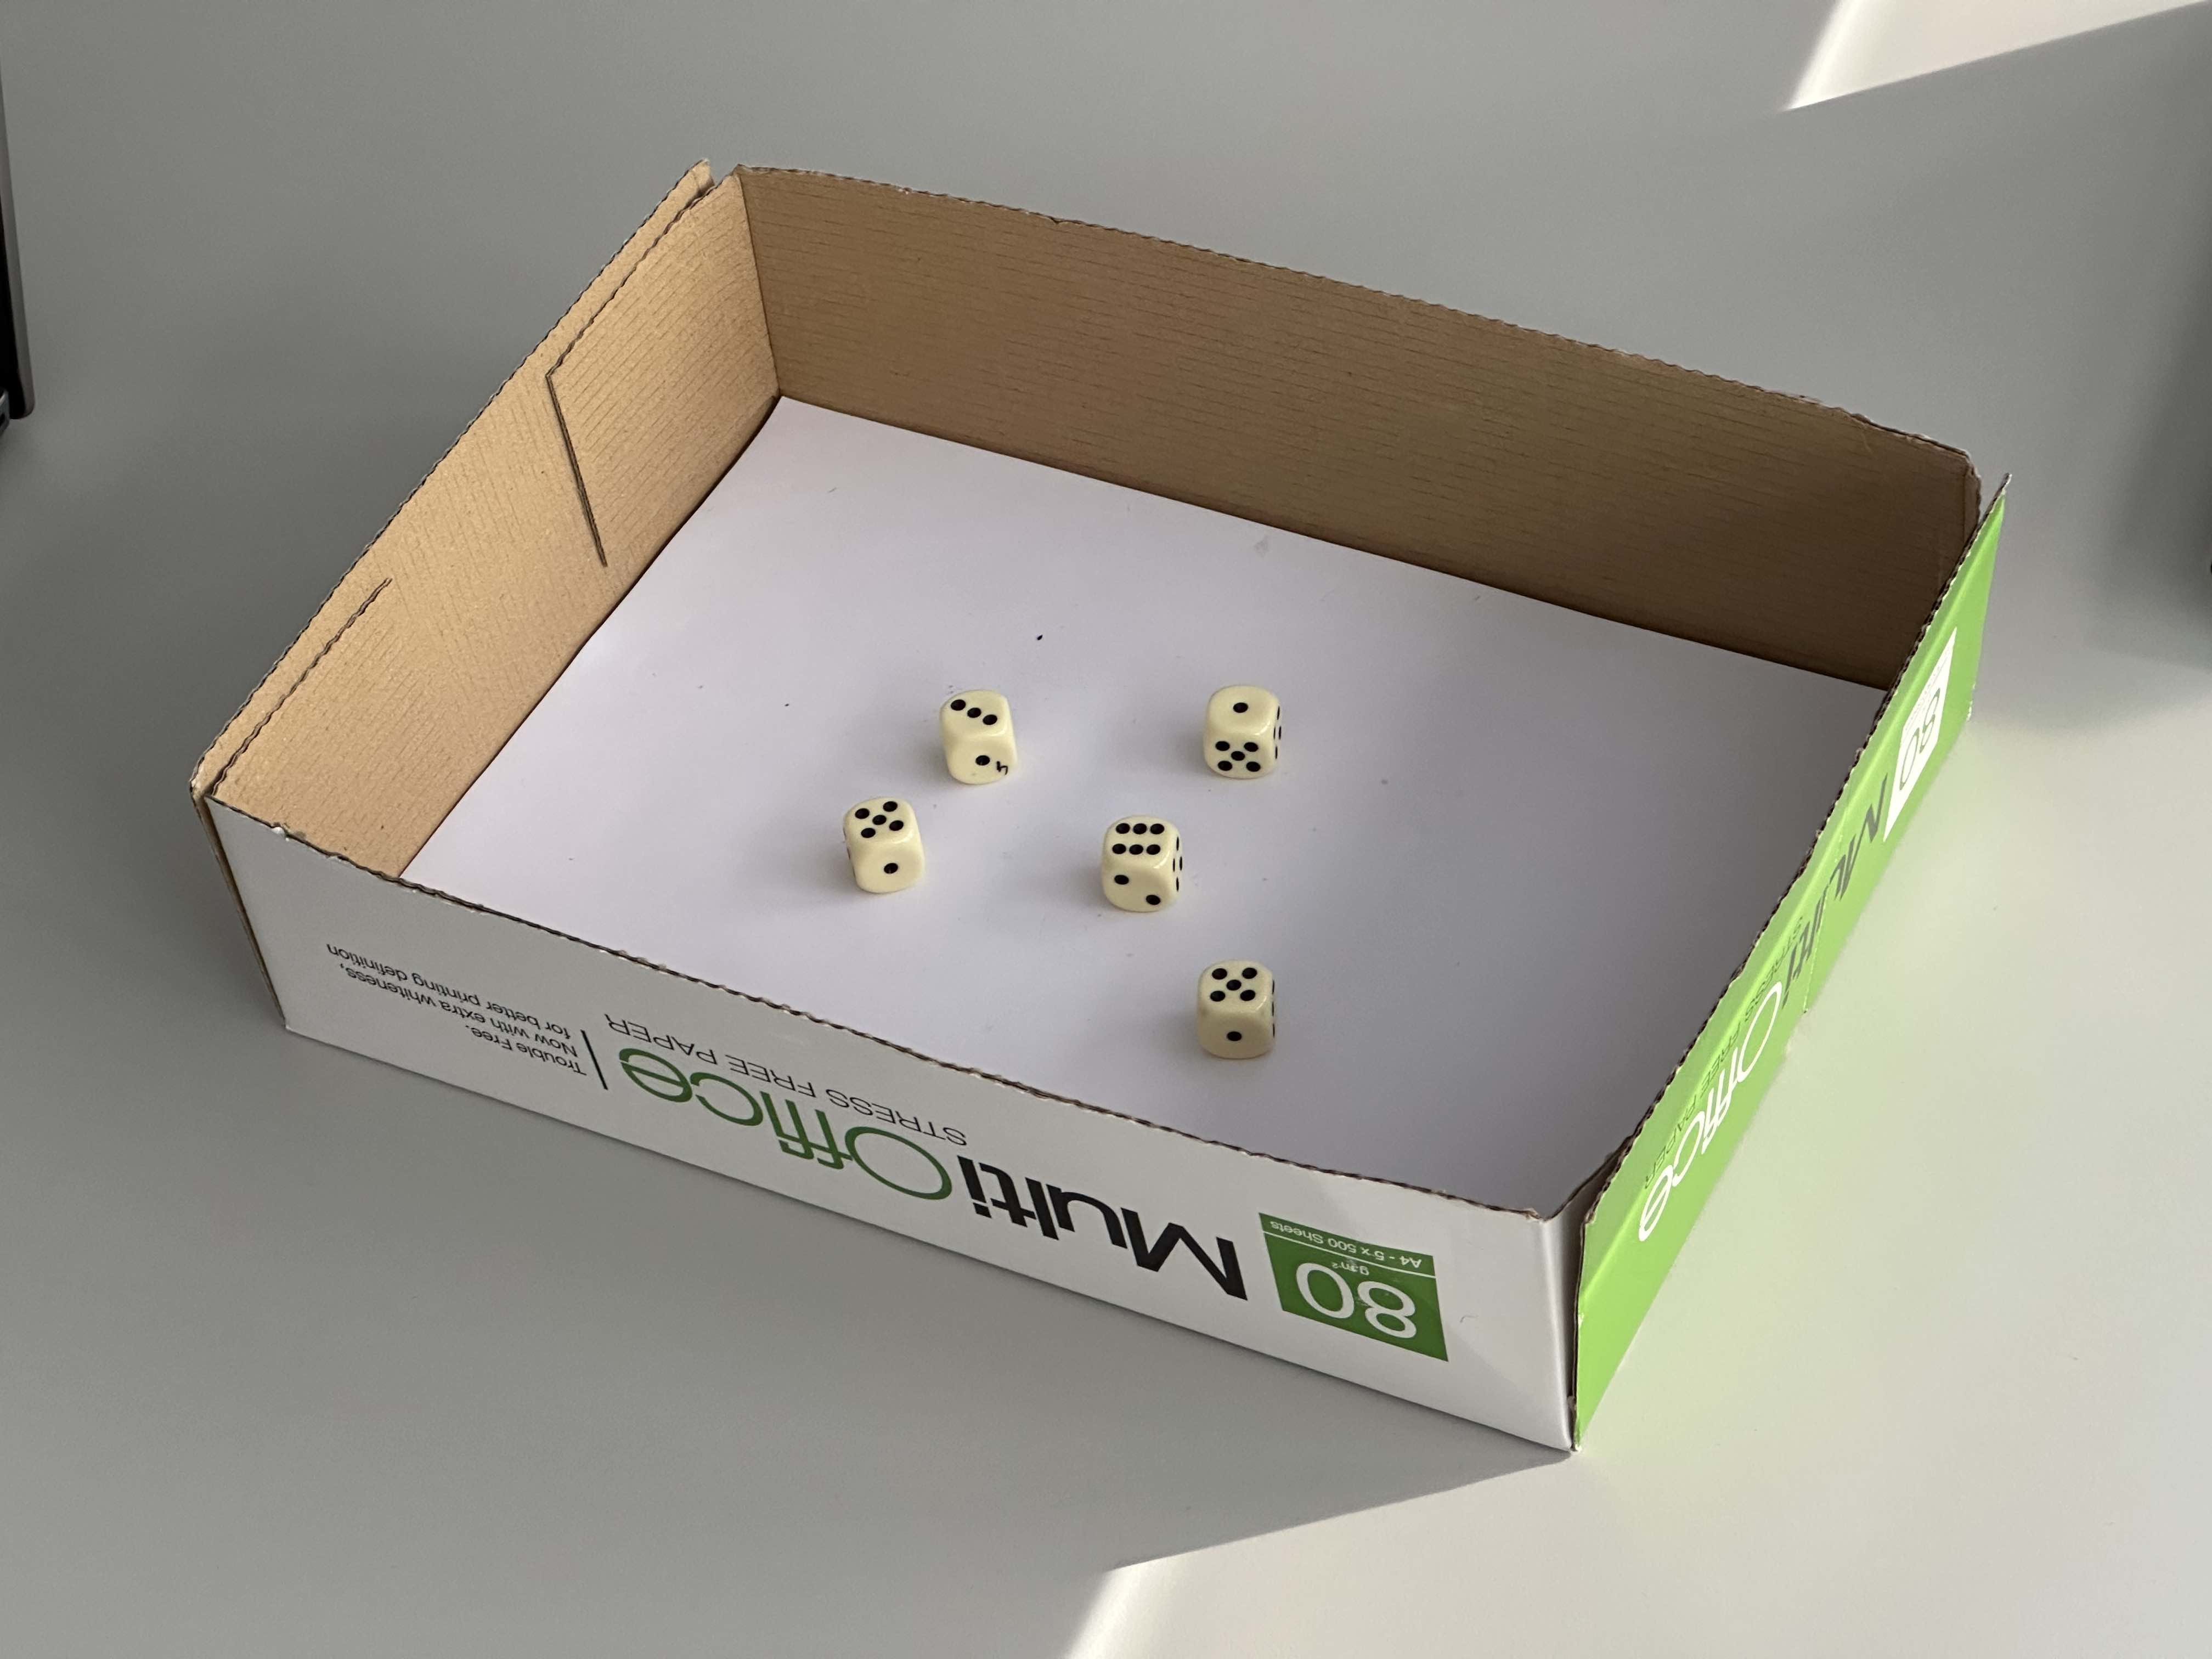
\includegraphics[width=0.5\textwidth]{bilder/IMG_7612.jpg}
    \caption{Würfelteller mit 5 Würfel}
    \label{Abb1}
\end{figure}

\subsection{Durchführung}
%//[x] Durchführung
% Wie wurde der Versuch durchgeführt bzw. ausgewertet?
Der Versuch wurde am 18. Oktober 2024 um ca. halb 12 im Raum P122 an der JKU Linz durchgeführt.
Für jeden Messvorgang wurden fünf Würfel gleichzeitig von der Hand in das Würfelteller geworfen. Dabei wurde jeder Würfel 
unabhängig von den anderen betrachtet. Anschließend wurden die Augenzahlen einzeln abgelesen, wobei die Reihenfolge außer 
Acht gelassen wurde. Die abgelesenen Werte wurden im direkten Anschluss an den Würfelvorgang im Laborprotokoll tabellarisch 
dokumentiert. Zur Überprüfung wird handschriftlich ein Histogramm gezeichnet. Es sollen dabei alle Würfel im Würfelteller 
landen und die Würfel so geworfen werden, dass das Würfelergebnis durch den Wurf nicht beeinflussbar ist.

Dieser Vorgang wurde insgesamt 80 mal, für 400 Werte wiederholt. Wobei zur Überprüfung nach 200 Messwerten in OriginPro 
2024 ein vorläufiges Histogramm erstellt wurde. 

\section{Messergebnisse und Auswertung}
%//[x] Messung
% Eigentliche Messung!
% Wie groß sind die Messunsicherheiten („Messfehler“)?
%//[x] TODO: Anführungszeichen unten
Die Messwerte sind dem auf \url{https://eln.jku.at/} zugänglichen bzw. angehängten Laborprotokoll \glqq Versuch_Würfeln_Laborprotokoll.pdf\grqq{} zu entnehmen.

%//[x] Auswertung
% evtl. Formeln, etc.
% auf richtiges Runden der Werte achten

Zur Auswertung werden zuerst die Werte für den statistischen Mittelwert $m$ und die statistische Standardabweichung 
$s$ berechnet und folglich die aus den Messungen hervorgehenden Stichprobenwerte für den Mittelwert $\mu$ und die 
Standardabweichung $\sigma$.

\begin{equation}
    \label{Gl1}
    m = \sum_{i=1}^{6} h_i \cdot x_i
\end{equation}

\begin{equation}
    \label{Gl2}
    s = \sqrt{\sum_{i=1}^{6} h_i\cdot(x_i - m)^2}
\end{equation}

\begin{equation}
    \label{Gl3}
    \mu = \frac{1}{N}\cdot \sum_{i=1}^{N} x_i
\end{equation}

\begin{equation}
    \label{Gl4}
    \sigma = \sqrt{\sum_{i=1}^{N} \frac{(x_i - \mu)^2}{N-1}}
\end{equation}

\begin{equation}
    \label{Gl5}
    \sigma_\mu = \sqrt{\frac{1}{N} \sum_{i=1}^{N} \frac{(x_i - \mu)^2}{N - 1}}
\end{equation}

\vspace{0,5cm}

Unter Anwendung von Gl. \ref{Gl1} ergibt sich $m=3,5$ und aus Gl. \ref{Gl2} folgt $s=1,71$.

Weiters wurde OriginPro 2024 verwendet, um den Mittelwert $\mu=3.54$ und die Standardabweichung $\sigma = 1,69$ der Messwerte
nach den Gleichungen \ref{Gl3} und \ref{Gl4} zu ermitteln.
Daraus folgt, dass die Grenzen des $1\sigma$ Vertrauensintervalls $3,54\pm1,69$ sind.
Die Ermittlung der Unsicherheit des Mittelwertes erfolgte in Excel nach Gleichung \ref{Gl5} und beträgt $\sigma_\mu\approx0,09$.

Diese Auswertung wird in Abbildung \ref{Abb2} dargestellt. Darin erkennbar ist außerdem eine Normalverteilung, die sich unter 
Annahme von gleichen $\mu$ und $\sigma$ ergibt. Man achte darauf, dass die Fläche unter der gesamten Normalverteilung so groß ist
wie die der Gleichverteilung, da die Summe der Wahrscheinlichkeiten aller Versuchsausgänge immer 100\% ist.

\begin{figure}[H]
    \label{Abb2}
    \centering
    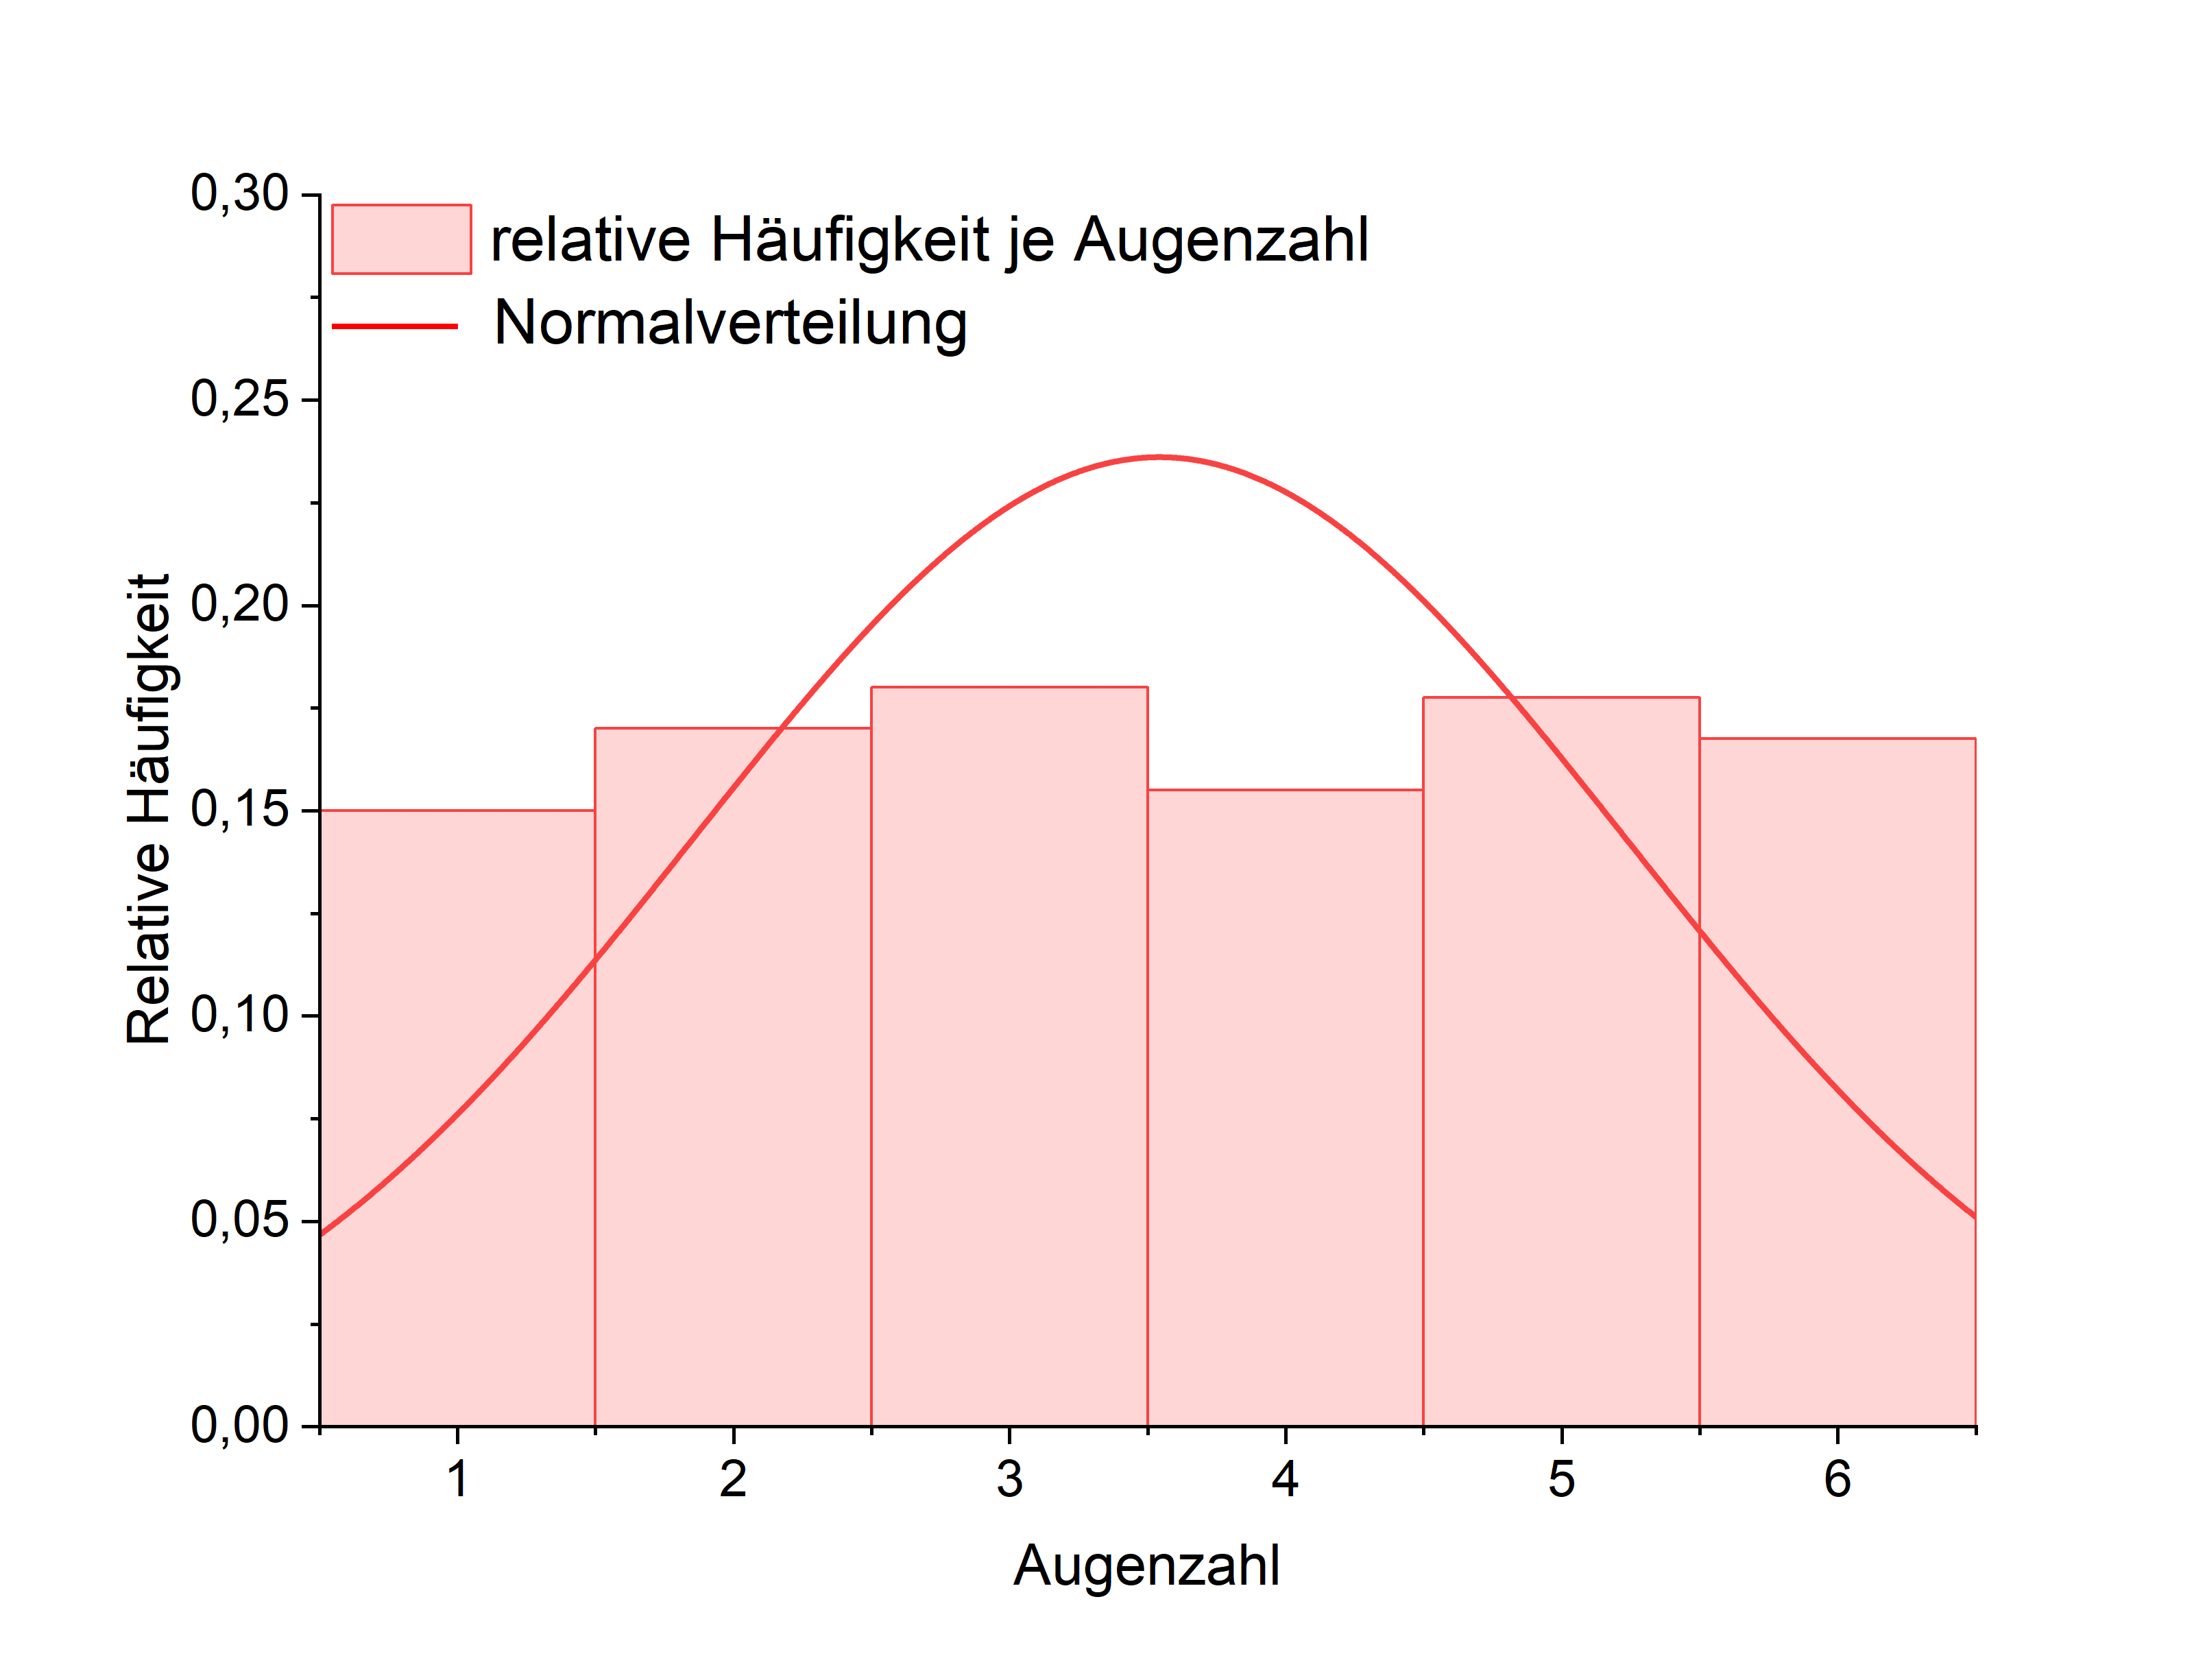
\includegraphics[width=\textwidth]{bilder/Histogramm.png}
    \caption{Histogramm der Messwerte}
\end{figure}

\section{Diskussion}
%//[x] Diskussion
% Wie vergleicht sich meine Messung mit anderen Messungen/Theorien?
% Ist der Messwert sinnvoll? Stimmt die Größenordnung?
% Wo wurden Fehler gemacht? Was kann man verbessern?
% Gegebenenfalls rekursiv auswerten oder nachmessen!
% ursprüngliche Fragestellung diskutieren
% zB Standardabweichung diskutieren, berechnete Größen nennen

Die durchgeführten Messungen wurden mit den theoretischen Erwartungswerten verglichen, und es zeigte sich, 
dass die gemessenen Werte weitgehend im Einklang damit stehen.

Die ursprüngliche Fragestellung, ob die gemessenen Werte eine bestimmte Verteilung aufweisen, kann 
durch den Vergleich mit einer Gleichverteilung beantwortet werden.
Die berechneten Größen, wie der Mittelwert des Experiments $\mu=3.54$ und die 
Standardabweichung des Experiments $\sigma = 1,69$, sind nahe and den theoretisch äquivalenten Werten $m=3,5$ 
und $s=1,71$.

Nach der Auswertung von 200 Messwerten wurde ein vorläufiges Histogramm aus den dokumentierten Daten 
erstellt und mit den handschriftlichen Notizen und dem handschriftlichen Histogramm, das nebenbei 
gezeichnet wurde, verglichen. Dies diente zur Überprüfung und frühen Erkennung von eventuellen 
systematischen Fehlerquellen. Dies wurde nach 400 Messwerten im Zuge der Auswertung wiederholt.

Zu diesem Zeitpunkt fiel auf, dass die Verteilung der Messwerte eine ähnliche Form aufwies wie die 
erwartete Gleichverteilung. Dies sieht aus, als deute es darauf hin, dass die Würfel nicht gezinkt wären, 
jedoch kann dies nicht eindeutig bestätigt werden, da für das Experiment immer fünf Würfel gleichzeitig
verwendet wurden. Es könnte erst eine bessere Aussage darüber gemacht werden, ob einer oder mehrere der Würfel gezinkt waren, 
wenn weitere Versuche gemacht werden würden. Diese Versuche würden jeweils immer nur einen einzelnen Würfel betrachten.
Selbst dann kann man nur Vermutungen anstellen und keine absoluten Aussagen treffen, da in einem endlichen Experiment 
ein gezinkter Würfel auch zufällig die gleichen Ergebnisse wie ein fairer Würfel liefern könnte, sowie ein fairer Würfel 
auch zufällig die gleichen Ergebnisse wie ein gezinkter Würfel liefern könnte.

Ein fairer Würfel hat für jede Seite die gleiche Wahrscheinlichkeit, nach oben zu zeigen. Diese Charakteristik 
der Häufigkeitsverteilung ist unter Anderem beeinflussbar durch eine nicht homogene Massenverteilung und einer vom 
regulären Würfel abweichende Form.

Eine höhere Zahl an Wiederholungen des Experiments sollte die relative Häufigkeit der einzelnen Augenzahlen
näher an die theoretischen Wahrscheinlichkeiten bringen, jedoch wurde nach 400 Messungen die Entscheidung getroffen,
dass diese Anzahl ausreichend ist, um die Fragestellung zu beantworten.

Zusammenfassend lässt sich sagen, dass die Messungen erfolgreich waren und die Ergebnisse 
mit den theoretischen Vorhersagen übereinstimmen. Es gibt jedoch Raum für Verbesserungen, 
insbesondere in Bezug auf das einzelne Überprüfen der Fairness der Würfel und die Erhöhung der Anzahl 
der Messungen.

\end{document}
